\documentclass[12pt,a4paper,UTF8]{article}
\usepackage{requirements}
\usepackage{environments}

\begin{document}

% Add your class number, student number, and programme name to this file.
% DO NOT edit anything else.
\fancyhead[L]{Project Title} % Setting the header
\fancyhead[R]{}

\label{cover}
\begin{titlepage}

    \begin{figure}[h]
    \centering
    \begin{minipage}{0.45\textwidth}
        
\includegraphics[width=\linewidth]{logo/logo_BUPT.jpg} 
    \end{minipage}\hfill
    \begin{minipage}{0.45\textwidth}
        
\includegraphics[width=\linewidth]{logo/logo_QM.png} 
    \end{minipage}
    \end{figure}

    \centering
    \vspace*{2cm}
    
    {\fontsize{25pt}{30pt}\selectfont Undergraduate Project Report \par}
    {\fontsize{25pt}{30pt}\selectfont 2024/25 \par}
    \vspace{1cm}
    {\fontsize{22pt}{30pt}\selectfont \textbf{Project Title} \par}

    
    \vfill
    \fontsize{16pt}{30pt}\selectfont
    \begin{tabular}{ll}
    Name: & Forename Surname \\
    School: & International School \\
    Class: & xxxxxxxxxxxx \\ % add your class number
    QMUL Student No.: & xxxxxxxxxxxx \\ % add your QM student number
    BUPT Student No.: & xxxxxxxxxxxx \\ % add your BUPT student number
    Programme: & xxxxxxxxx \\ % add your programme number
    \end{tabular}
    \vspace{4cm}
    
    \textbf{Date: dd-mm-yyyy} % enter the date
    \vspace{1cm}
\end{titlepage}

\tableofcontents
\thispagestyle{fancy}
%%%%%%%%%%%%%%%%%%%%%%%%%%%%%%%%%%%%%%%%%%%%%%%%%%%%%%%%%%%%%%%
% Your report content starts here
% The commands below defines the structure of your report
% The \input{...} command includes the content of the specified file (e.g., contents/abstract.tex) into the document
% to edit the content, locate and modify the corresponding file.
\linespread{1.5} % Set line spacing to 1.5x

\newpage
\onehalfspacing
\addcontentsline{toc}{section}{\textit{Abstract}}
{\fontsize{16pt}{30pt}\selectfont \noindent\textbf{Abstract}}
\vspace{0.5cm}
{\fontsize{12pt}{18pt}\selectfont
% replace the paragraph below with your abstract

The abstract should be a short overview of the whole report (200-300 words maximum). It should give the reader enough information about your entire project to know what you have tried to do and whether you were successful.

}
\vspace{0.5cm}
\addcontentsline{toc}{section}{\textit{Keywords}}
{\fontsize{16pt}{30pt}\selectfont \noindent\textbf{Keywords}}
\vspace{0.5cm}
{\fontsize{12pt}{18pt}\selectfont
% replace the paragraph below with your keywords

Keyword 1, Keyword 2, Keyword 3 (List of Keywords, separated by commas)

}



\newpage
\onehalfspacing
{\fontsize{16pt}{30pt}\selectfont \noindent\textbf{摘要}}
\vspace{0.7cm}
{\fontsize{12pt}{18pt}\selectfont
% replace the paragraph below with your abstract

This is the Chinese translation of the Abstract.

}
\vspace{1.0cm}
{\fontsize{16pt}{30pt}\selectfont \noindent\textbf{关键词}}
\vspace{0.7cm}
{\fontsize{12pt}{18pt}\selectfont
% replace the paragraph below with your keywords

This is the Chinese translation of the Keywords, separated by commas and following the same sequence.

}


\newpage
\section*{Chapter 1: Introduction}
\setcounter{section}{1} \setcounter{subsection}{0}
\addcontentsline{toc}{section}{\textit{Chapter 1: Introduction}}

The \textit{Introduction} is one of the most important parts of your report as it gives a brief overview that will make the reader understand (i) what you set out to do and (ii) what you achieved. Many readers will read the \textit{Introduction} first and then the  \textit{Conclusions} to get an overview before reading the detail – so it is important that both sections are very carefully written.

It is very important that \textit{Introduction} introduces the \textbf{report} and the \textbf{project} – it is not there to introduce the subject in general.

There are no rules on how to write an introduction, but it should include what the project is about, give \textit{a very short description} of the technical context in which the project is carried out and explain the motivation for the work. If you are doing an implementation project it must explain what functionality the system \textbf{realises}, and if you are doing a research project what is the novelty of the approach used. 

Very importantly, it should clearly indicate what you have done for the project. 

A good introduction should be no more than 4 pages.
\subsection{Format}
\subsubsection{Format for headings}
Format for level 1, 2 and 3 headings is given in this template; just choose the relevant style from the format list.

\subsubsection{Format for body text}
Font Times New Roman, Font size should be 12pt, 1.5 line spacing in and justified. Do not indent the first line.
% the default setting in LaTeX already satisfies the above theme.

\subsubsection{Format for equations}
Equations should be centred with a numbered caption on the right; an example is below:
\begin{equation}
I_{\,i, own}=P_{\,total, j} \cdot \gamma_{\,i, j} - P_{\,i,recv}
\end{equation}

\subsubsection{Format for figures}

Figures should be centred and followed by captions. Captions should be centred, 10pt font 
Times New Roman Bold. Use automatic numbering without chapter number for captions. Select “Caption” from Styles and Formatting to format captions.

Whenever you include a figure in your document you must reference it in the text e.g. this is a reference to Figure\ref{fig:examplefig}.

When presenting graphs, make sure you label the axes and include units where applicable. Also include a legend (i.e. key) where appropriate.

\begin{figure}[h]
\centering
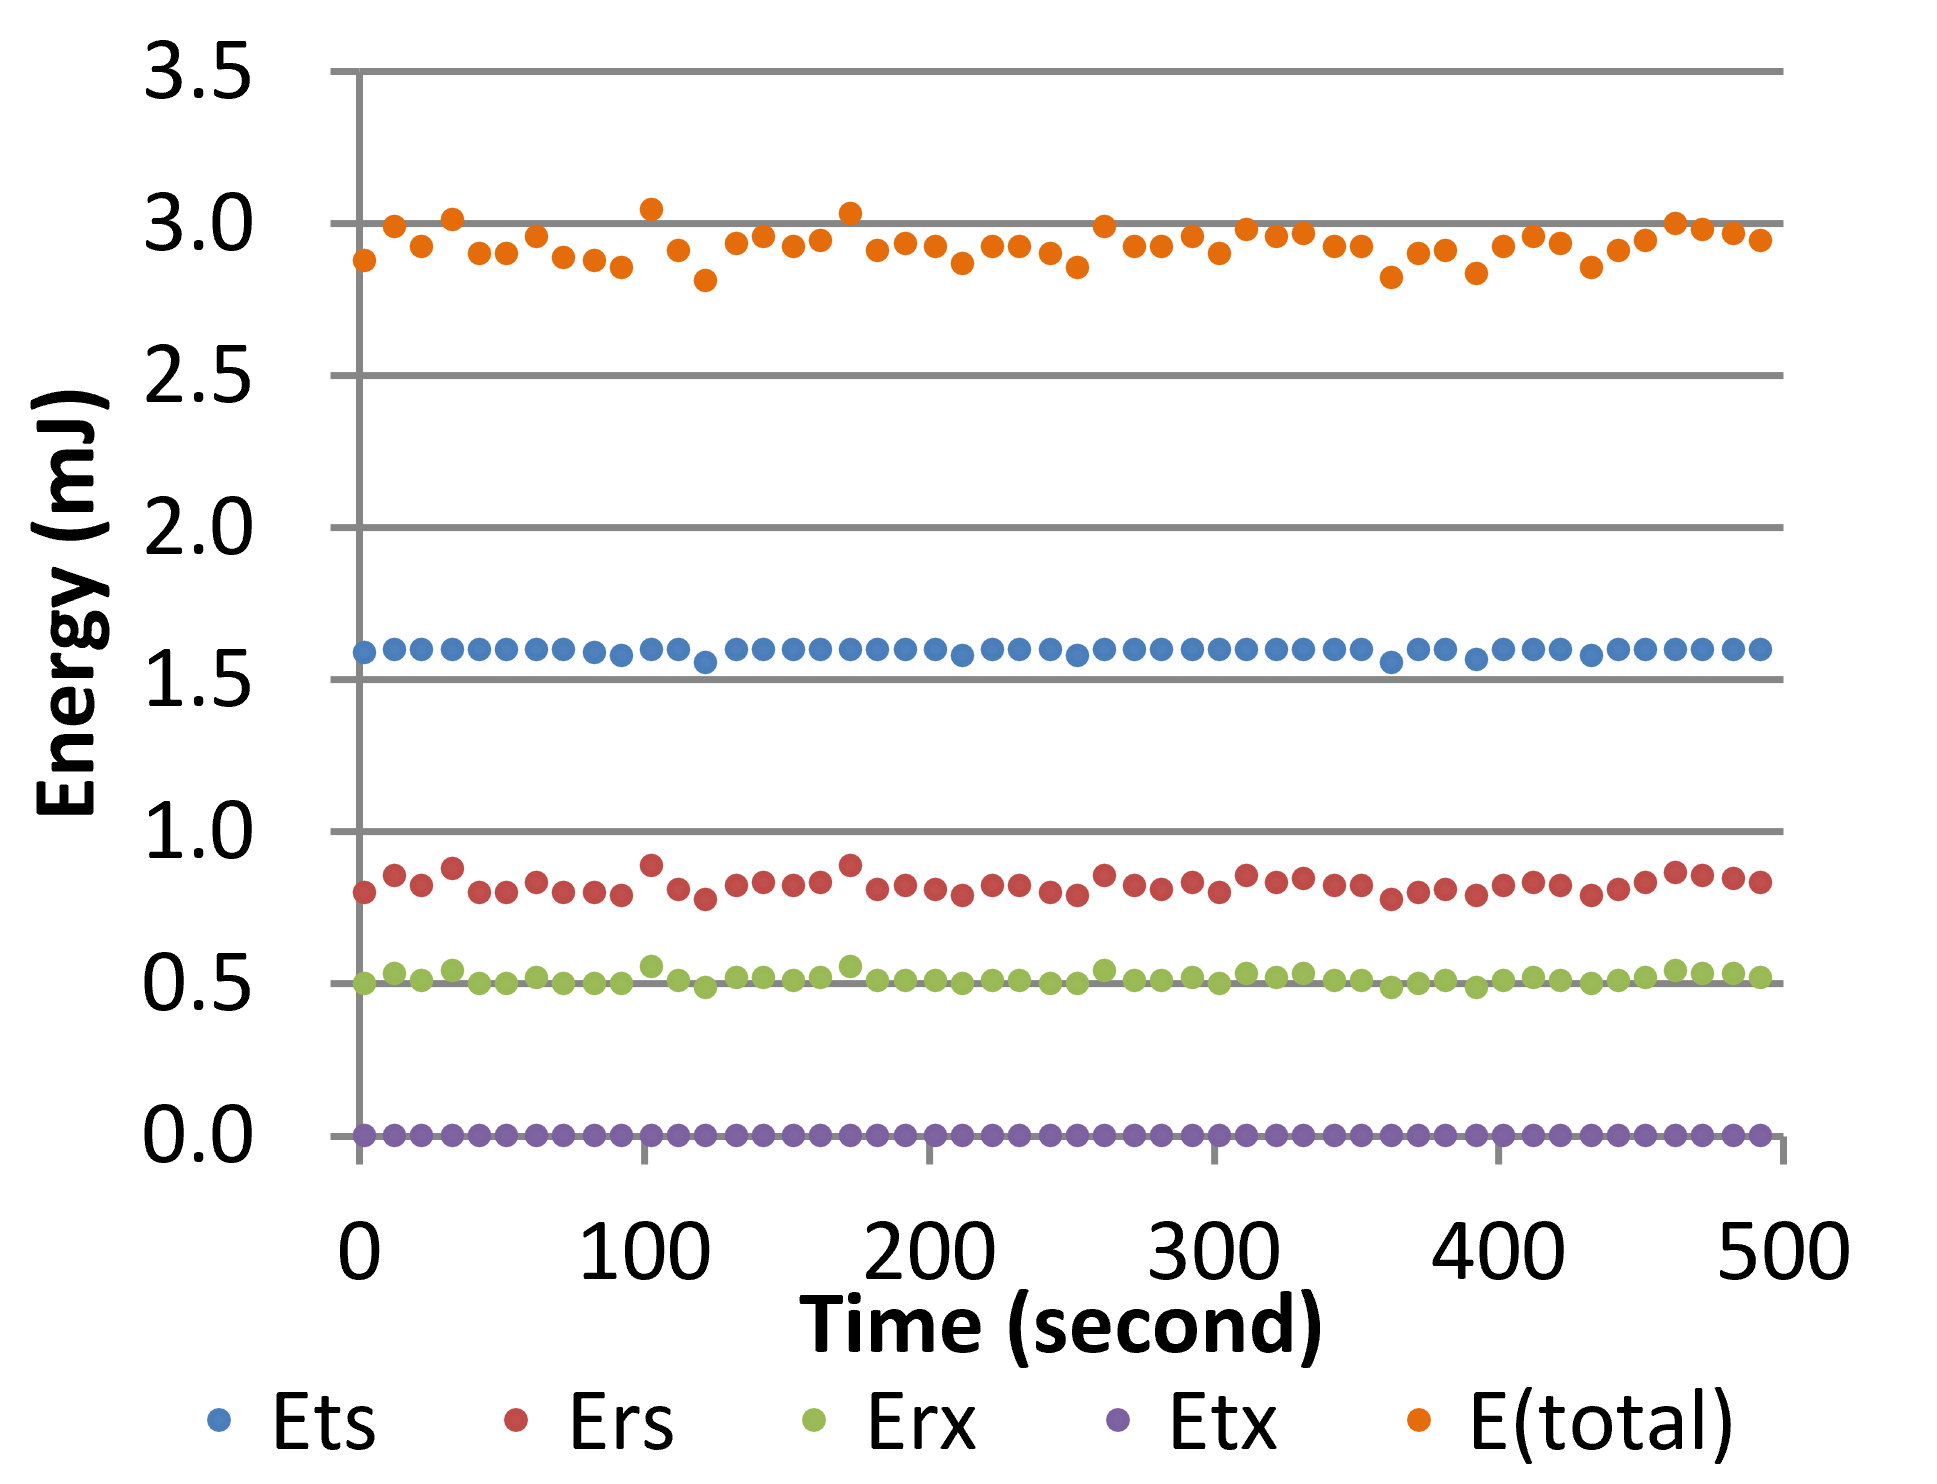
\includegraphics[width=10cm]{figures/examplefig.PNG}
\caption{Comparison of energy components}
\label{fig:examplefig}
\end{figure}

\subsubsection{Format for Tables}
Unlike figures, the caption for a table should be before the table; Table\ref{table:exampletable} shows an example of the correct layout.


\begin{table}[h]  
  \centering  
  \begin{spacing}{1.35}  
  \caption{Example Table}\vspace{0.7em}
  \label{table:exampletable} 
    \begin{tabular}{|p{4cm}|p{4cm}|p{4cm}|}   
    \hline
     & & \\  
    \hline
     & & \\
    \hline
     & & \\
    \hline
    \end{tabular}
  \end{spacing}
\end{table}


\newpage
\section*{Chapter 2: Background}
\setcounter{section}{2} \setcounter{subsection}{0}
\addcontentsline{toc}{section}{\textit{Chapter 2: Background}}


In this part of the report, you should give all the relevant background information about your project. Remember that your reader will not necessarily know the background technology you are using, so it is worthwhile to let them know.

Also if your project is a research project, this is a good place to put down the related work or state of the art in the area – what the others have done? And why your research is novel?

But don't make the background too long with every detail. It should be relevant to your project, with all the necessary information, written nicely and crisply.


\newpage
\section*{Chapter 3: Design and Implementation}
\setcounter{section}{3} \setcounter{subsection}{0}
\addcontentsline{toc}{section}{\textit{Chapter 3: Design and Implementation}}

Normally there will be a part about the design and implementation of the system, especially for an implementation type of project. However, every project has its unique phases so you should talk to your supervisor about it.


\newpage
\section*{Chapter 4: Results and Discussion}
\setcounter{section}{4} \setcounter{subsection}{0}
\addcontentsline{toc}{section}{\textit{Chapter 4: Results and Discussion}}

Most projects will have results, especially for a research project. But again you should talk to your supervisor about it.


\newpage
\section*{Chapter 5: Conclusion and Further Work}
\setcounter{section}{5} \setcounter{subsection}{0}
\addcontentsline{toc}{section}{\textit{Chapter 5: Conclusion and Further Work}}

The conclusion is an important part of the report, as it states what you have done for the project.

\subsection{Conclusion}
It concludes the findings of your research or the outcome of implementing a system. A good conclusion will NOT repeat what you have done, but set out the achievements very crisply.

\subsection{Reflection}
This chapter should include a reflection statement for your project. You should critically reflect upon the technical skills developed, new knowledge gained, and lessons learnt on the project journey. You are encouraged to include reflections on broader ethical, social, legal, and environmental issues, allied with good professional practice and behaviour you have adopted in conducting your project.

\subsection{Further work}
Further work can be the next step of your research, or some functionality that can be added to the implementation to make it more practical.

\vspace{\baselineskip}
\noindent\textbf{NOTE: The maximum length of the report up to here is 50 pages.}


\newpage
\addcontentsline{toc}{section}{\textit{References}}
\bibliography{reference}
% Referencing in LaTeX: A Quick Guide
% ----------------------------------
% 1. Add References:
%    - Open the existing 'references.bib' file.
%    - Add new references in BibTeX format.
%    - Example BibTeX entry for a journal article:
%      @article{newkey,
%        author  = {Author Name},
%        title   = {Article Title},
%        journal = {Journal Name},
%        year    = {Year},
%        volume  = {Volume},
%        pages   = {Pages}
%      }

% 2. Cite References Inline:
%    - Use the \cite{key} command in your document, where 'key' is the unique identifier from the BibTeX entry.
%    - Example (try uncomment the following line and run compile to see the result):
     % This method was proposed in \cite{basar2019,mouftah2018,qmul2024,saputra2019}.

%%%%%%%% delete the following paragraph in your report.%%%%%%%%
Everything you cite from other sources should be properly referenced. The QMUL Faculty of Science and Engineering has identified the Vancouver referencing style (and its variations) as the recommended styles for project reports. Details about the referencing style and examples can be found online. \href{https://www.qmul.ac.uk/library/academic-skills/referencing-hub/referencing-guides-and-resources}{https://www.qmul.ac.uk/library/academic-skills/referencing-hub/referencing-guides-and-resources}

It is recommended to prepare the references with a reference management software, such as \href{https://www.qmul.ac.uk/library/academic-skills/endnote/endnote-online/}{EndNote} or \href{https://qmplus.qmul.ac.uk/mod/book/view.php?id=653429&chapterid=66169}{Zotero} to automate some of the processes of collecting, managing and using references. Queen Mary Library Services promote the use of \href{http://ezproxy.library.qmul.ac.uk/login?url=https://www.citethemrightonline.com/}{Cite Them Right Online} (login required) as a tool to support Queen Mary students in their referencing.

Here are some examples in Vancouver referencing style:

\textbf{Book Chapters:}

Mouftah HT, Erol-Kantarci M, Husain Rehmani M. Transportation and Power Grid in Smart Cities: Communication Networks and Services. 1 ed: Wiley; 2018.

\textbf{Journal Articles:}

Basar E, Di Renzo M, De Rosny J, Debbah M, Alouini MS, Zhang R. Wireless Communications Through Reconfigurable Intelligent Surfaces. IEEE Access. 2019;7:116753–73.

\textbf{Conference Papers:}

Saputra YM, Hoang DT, Nguyen DN, Dutkiewicz E, Mueck MD, Srikanteswara S. Energy Demand Prediction with Federated Learning for Electric Vehicle Networks. 2019 IEEE Global Communications Conference (GLOBECOM). Waikoloa, HI, USA: IEEE; 2019. p. 1–6.

\textbf{Online sources:}

Queen Mary University of London. Student Guide to Generative AI [Internet]. 2024 [cited 15 Jan 2025]. Available from: \href{https://www.qmul.ac.uk/library/academic-skills/student-guide-to-generative-ai/}{https://www.qmul.ac.uk/library/academic-skills/student-guide-to-generative-ai/}
%%%%%%%%%%% delete up to here%%%%%%%%%%%%



\newpage
\addcontentsline{toc}{section}{\textit{Acknowledgment}}
\section*{Acknowledgment}
\vspace{-\baselineskip}
{\fontsize{12pt}{18pt}\selectfont 

Give your acknowledgment to people who helped you during the project here. Maximum length of this section is 1 page. You may thank your supervisor but \textcolor{red}{DO NOT MENTION YOUR SUPERVISOR’S NAME HERE due to the blind marking policy}.

}

%%%%%%%%%%%%%%%%%%%%%%%%%%%%%%%%%%%%%%%%%%%%%%%%%%%%%%%%%%%%%%
% Here's your appendix section
\newpage
\section*{Appendices}
\addcontentsline{toc}{section}{\textit{Appendices}} \vspace{-1em}
\subsection*{Disclaimer}
\addcontentsline{toc}{subsection}{Disclaimer}
\raggedright \vspace{-1em}
This report is submitted as part requirement for the undergraduate degree programme at  Queen Mary University of London, and Beijing University of Posts and Telecommunications. It is the product of my own labour except where indicated in the text. The report may be  freely copied and distributed provided the source is acknowledged.

% You only need to fill in your information as below
\hspace*{\fill}

BUPT No.:

QMUL No.:

Full Name (Pin Yin):

Full Name (Chinese):

\hspace*{\fill}

Signature:

\hspace*{\fill}

Date:DD-MM-YYYY


\newpage
\subsection*{Project specification}
\addcontentsline{toc}{subsection}{Project specification}

\raggedright
Include your project specification, part 1 and part 2 here. It must be the final version\newline submitted to QMPlus. % remove this paragraph in your thesis and follow the instruction below


% Instruction: You need to include it as a pdf file, with the following steps
% 1. Save the file as a pdf
% 2. Upload/Copy the pdf to the same directory as this file
% 3. Uncomment the command at the bottom
% 4. Change 'your_path' to the path of the uploaded pdf

% \includepdf[pages=-, pagecommand={},clip]{your_path.pdf}

\newpage
\input{appendices/earlyTermProgressReport}

\newpage
\input{appendices/midTermProgressReport}

\newpage
\subsection*{Supervision log}
\addcontentsline{toc}{subsection}{Supervision log}

Include your project supervision log here.% remove this paragraph in your thesis and follow the instruction below


% Instruction: You need to include it as a pdf file, with the following steps
% 1. Save the file as a pdf
% 2. Upload/Copy the pdf to the same directory as this file
% 3. Uncomment the command at the bottom
% 4. Change 'your_path' to the path of the uploaded pdf

% \includepdf[pages=-, pagecommand={},clip]{your_path.pdf}

\newpage
\input{appendices/additionalAppendices}

%%%%%%%%%%%%%%%%%%%%%%%%%%%%%%%%%%%%%%%%%%%%%%%%%%%%%%%%%%%%%%%
% The final section on "Risk and environmental impact assessment"
\newpage
\addcontentsline{toc}{section}{\textit{Risk and Environmental Impact Assessment}}
\section*{Risk and Environmental Impact Assessment}

Please refer to the project handbook section 3.6.12



\end{document}
